\section{Method: The VIGIL Framework}
\label{sec:framework}
\subsection{Overview}

VIGIL comprises two layers. A sensing pipeline discovers AI-litigation filings in CourtListener/RECAP~\citep{courtlistener2023} and legal news and converts them into case records; this engineering infrastructure is documented in Appendix~\ref{app:impl} (architecture in Figure~\ref{fig:vigil_arch}). The remainder of this section describes the evaluated NLP components in order: LegalRisk-RAG (\S\ref{sec:legalrag}), the goal-conditioned agentic loop (\S\ref{sec:agentic_loop}), the temporal precedent graph (\S\ref{sec:tpg}), and the PLRE decision procedure (\S\ref{sec:plre}).

\subsection{LegalRisk-RAG}
\label{sec:legalrag}

The LegalRisk-RAG pipeline adapts standard RAG to legal text in three respects. \textbf{Chunking} segments documents at logical structural boundaries---numbered claims, ``WHEREFORE'' clauses, section headings---rather than fixed token windows; each chunk retains a metadata header (case identifier, filing date, court level, section type). \textbf{Embedding}: we compared a dense retriever~\citep{karpukhin2020dense} (\texttt{text-embedding-3-large}), RECAP-tuned LegalBERT~\citep{chalkidis2020legalbert}, and a hybrid BM25 + neural re-ranker on a 200-pair development set; the hybrid performed best and is the default (Table~\ref{tab:retriever_ablation}, appendix). \textbf{Dynamic context expansion (precedent chaining)}: when a retrieved chunk references a prior case (e.g., \emph{Authors Guild v.\ Google}), the pipeline appends that opinion as secondary context and queries the temporal precedent graph for subsequent treatment, so that the Analyzer receives both semantic neighbors and validity metadata (cited positively, narrowed, superseded, or overruled at the filing date).

\subsection{Goal-Conditioned Agentic Loop}
\label{sec:agentic_loop}

The four specialized agents and the central Goal Checker operate as in Algorithm~\ref{alg:vigil_loop}. The \textbf{Planner} decomposes unmet sub-goals into ordered retrieval/analysis sub-tasks; the \textbf{Retriever} runs LegalRisk-RAG queries and reformulates via legal entity term expansion when $\mathcal{G}_{\text{evidence}}$ is unmet; the \textbf{Analyzer} computes $\text{RiskScore}(d_i, P, C)$, clusters evidence, and maps clusters to a risk taxonomy (Training Data, Output Reproduction, API Misuse, Model Weights); the \textbf{Goal Checker} evaluates $\mathcal{G}(R_t)$ after each pass and returns machine-readable residuals such as \texttt{missing(valid-authority, DMCA, output-CMI, NDCA, 2025-02)}; the Planner converts these critiques into expanded entity/date/theory queries; and the \textbf{Reporter} assembles the risk register, per-risk evidence with citations, and mitigation guidance.

\subsection{Temporal Precedent Graph}
\label{sec:tpg}

VIGIL's central component is a treatment layer that determines \emph{when} each authority ceases to be operative; a simple retrieval-time gate then applies it. The layer is realized as a temporal precedent graph $\mathcal{P}_t=(V,E_t)$. Each node $v\in V$ denotes a case, order, or doctrinal rule and stores jurisdiction, court level, issue tags, filing and decision dates, and a validity interval $[s_v,e_v)$, where $e_v$ remains open unless the node is later vacated, overruled, or superseded; material narrowing instead lowers its treatment weight. Directed edges encode treatment relations: \textsc{cites}, \textsc{distinguishes}, \textsc{narrows}, \textsc{supersedes}, and \textsc{overrules}. Retrieval for a query at date $t_q$ first obtains semantically relevant candidates and then applies validity gating:
\begin{equation}
\label{eq:tpg_score}
\begin{split}
  \mathrm{score}(v,q,t_q)={}&\mathrm{sim}(v,q)\cdot \mathbf{1}[s_v\!\le\! t_q\!<\! e_v]\\
  &\cdot w(\mathrm{treat}(v,t_q)).
\end{split}
\end{equation}
Here $w(\cdot)$ is a fixed monotone schedule: positively treated or still-open authorities (\textsc{cites} with positive/neutral polarity, or no negative treatment) receive weight $1.0$; \emph{cautionary} authorities---those labeled \textsc{distinguishes} or bearing weak negative polarity without interval closure---receive $0.75$; material \textsc{narrows} receives $0.50$; fully closed (overruled or superseded) authorities are already excluded by the indicator. The operator separates legal authority from topical similarity: a stale but lexically close case may still appear as context, yet it cannot support a risk decision without passing the validity check. Equation~\eqref{eq:tpg_score} is therefore a constrained retrieval operator over $(q,t_q)$: a host retriever scores semantic relevance as usual, and PLRE receives only support whose legal status remains operative at $t_q$. Unlike a learned temporal re-ranker (which can still rank closed authority highly) or a post-hoc citator warning applied after evidence is selected, the gate hard-filters support before generation; we leave a head-to-head re-ranker baseline to future work.

\begin{figure}[t]
\centering
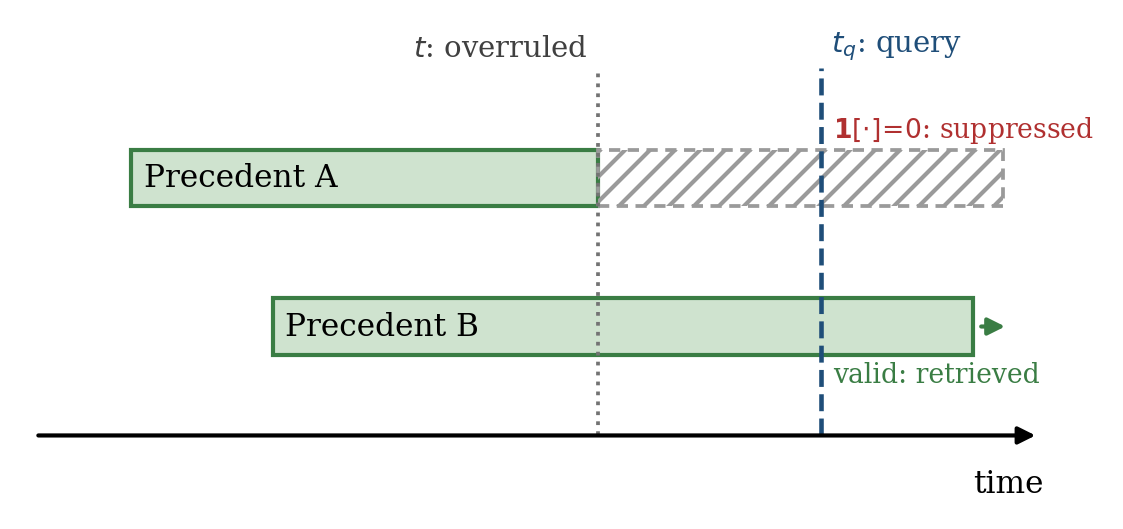
\includegraphics[width=0.99\linewidth]{fig_tpg.png}
\caption{Validity gating (Eq.~\eqref{eq:tpg_score}). An overruling at $t$ closes Precedent~A, so a query at $t_q\!>\!t$ zeroes its indicator and suppresses it despite lexical similarity, while still-open Precedent~B is retrieved---the time-valid distinction the RQ3 ablation isolates.}
\label{fig:tpg_mech}
\end{figure}

\paragraph{Why not a date filter?} Once intervals are known, Eq.~\eqref{eq:tpg_score} is a metadata filter any vector store can apply. The difficulty is upstream and conceptual: $e_v$ is set by \emph{later} documents that overrule, supersede, or narrow $v$, so it is not recoverable from $v$'s own filing date. A pure recency or document-date filter therefore cannot implement the same operator; the empirical question is whether treatment edges can be extracted reliably enough to use. Table~\ref{tab:edge_summary} addresses that question: negative-treatment micro-F1 is 0.80 on 600 gold spans and 0.81 against a commercial citator (Protocol~P2; missed-action rate 20.4\%; 3.8\% of held-out PLRE pairs flip after citator correction). Per-relation tables, error propagation, and a weaker regex baseline appear in Appendix~\ref{app:edge_extraction}, \ref{app:p2}.

\begin{table}[t]
\centering
\caption{Treatment-layer validation (neg.-treatment micro over \textsc{overrules}/\textsc{supersedes}/material \textsc{narrows}).}
\label{tab:edge_summary}
\small
\setlength{\tabcolsep}{4pt}
\begin{tabular}{l c c c}
\toprule
\textbf{Reference} & \textbf{P} & \textbf{R} & \textbf{F1} \\
\midrule
Gold spans ($n{=}600$)   & 0.84 & 0.77 & 0.80 \\
Citator (Protocol~P2)    & 0.83 & 0.80 & 0.81 \\
\bottomrule
\end{tabular}
\end{table}

\paragraph{Graph construction.} Nodes are induced from CourtListener/RECAP with intervals initialized to $[s_v,\infty)$. Edges are extracted by a citation-span detector plus an LLM classifier (GPT-4o, $T{=}0$; distinct from the controller's $T{=}0.2$); interval-closing edges must be anchored to a detected span, decision date, and source document, and gold evaluation uses spans held out from prompts. A confirmed \textsc{overrules}/\textsc{supersedes} edge at $t$ sets $e_v\!\leftarrow\!t$; material \textsc{narrows} sets $w{=}0.50$ from $t$. The graph has 1{,}812 nodes and 4{,}760 edges.

Low-confidence negative-treatment edges are routed to human review rather than auto-closing intervals; downstream effects of missed closures are audited in Table~\ref{tab:edge_sensitivity}.

\subsection{PLRE Decision Procedure}
\label{sec:plre}

We cast product--litigation alignment as a risk-entailment task. Given a product spec $P$ with attributes $\{p_1,\dots,p_m\}$ (training-data sources, collection method, output modality, architecture, deployment context, and capability claims), a legal-risk theory $T_j$, and a query date $t_q$, PLRE predicts:
\begin{equation}
  y_{ij}=\mathbf{1}[P,p_i,\mathcal{P}_{t_q} \models T_j].
\end{equation}
\begin{table}[t]
\centering
\caption{Schematic PLRE instances (illustrative; not drawn from VIGIL-Dataset). The same attribute--theory pair can be positive or negative depending on whether its supporting authority is still operative at $t_q$.}
\label{tab:plre_example}
\small
\setlength{\tabcolsep}{3pt}
\resizebox{\columnwidth}{!}{%
\begin{tabular}{p{2.3cm} p{2.2cm} p{2.4cm} c}
\toprule
\textbf{Attribute $p_i$} & \textbf{Theory $T_j$} & \textbf{Support at $t_q$} & $y_{ij}$ \\
\midrule
web-scale image scraping for training & training-data copyright infringement & operative authority on unlicensed training copies & 1 \\
\addlinespace
same & same & only authority whose interval closed before $t_q$ (stale distractor) & 0 \\
\addlinespace
output filter removes copyright-management information & DMCA \S1202 (output CMI) & no authority in the query's jurisdiction & 0 \\
\bottomrule
\end{tabular}%
}
\end{table}

Table~\ref{tab:plre_example} provides schematic instances. Unlike symmetric similarity, PLRE is directional: an attribute such as ``web-scale image scraping'' can support exposure to a training-data copyright theory, whereas the inverse relation is not meaningful. Unlike standard legal textual entailment, the premise incorporates product attributes and the entailment relation is conditioned on time-valid precedent. A pair $(p_i,T_j)$ is promoted to the risk register only when (i)~the entailment score exceeds the validation-set threshold, (ii)~the top supporting precedents remain valid at $t_q$, and (iii)~the report includes mitigation text grounded in at least three cited authorities when available.

PLRE gold labels are constructed from anonymized product-attribute cards and docket-grounded theory cards. Annotators judge a directional pair as positive only when the product attribute, legal theory, query date, and at least one valid supporting authority jointly establish exposure; negative pairs comprise ordinary mismatches and stale-authority distractors. Critically, the validity judgment encoded in the labels is produced by annotators reading docket and opinion text, \emph{independently of VIGIL's automatically extracted treatment graph}, so the gate must recover label validity rather than presuppose it. An extractor-independent re-check of these validity judgments against an authoritative citator forms the downstream link of Protocol~P2. Product archetypes are tracked in the split manifest, and year and litigation type are stratified to reduce temporal and topical leakage.

The formulation is system-agnostic: PLRE is directional entailment subject to an exogenous, time-indexed support constraint, and any system can be evaluated on it. It is more demanding than ordinary legal NLI because a model must align engineering terms with legal predicates \emph{and} reject stale yet lexically attractive precedent.
